	
\question [20] A figura a seguir mostra a curva de aquecimento de uma amostra de \SI{400}{\gram} de uma substância hipotética, inicialmente a \SI{15}{\celsius}, no estado sólido, em função da quantidade de calor que esta recebe.\\

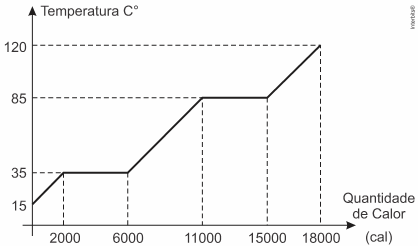
\includegraphics[width=0.6\linewidth]{provas/2ano3bim2021/ImagemQ2}\\

Determine o valor aproximado do calor latente de vaporização da substância, em cal/g.

	\begin{EnvUplevel}
		\begin{oneparchoices}
			\choice 10
			\choice 20 
			\choice 30   
			\choice 40  
			\choice 50
		\end{oneparchoices}
	\end{EnvUplevel}
\vspace{4cm}

\question [20] A exposição do corpo humano a baixas temperaturas pode causar danos à saúde. Por esse motivo, surfistas utilizam roupas especiais quando praticam seu esporte em águas muito frias. A função dessas roupas é:

	\begin{EnvUplevel}
		\begin{choices}
		\choice transferir calor do meio ambiente para o corpo.
		\choice armazenar calor e fornecê-lo de volta ao corpo.   
		\choice diminuir o fluxo de calor do corpo para o meio ambiente.   
		\choice estimular a produção de calor pelo corpo.     
		\choice facilitar a dissipação do calor produzido pelo corpo.
		\end{choices}
	\end{EnvUplevel}


\vspace{2cm}

\question [20] Um objeto de massa $m=$\SI{1}{\kilogram} recebe uma certa quantidade de calor $Q$ e, com isso, sofre uma variação de temperatura $\Delta T$. A relação entre $T$ e $Q$ está representada no gráfico a seguir. 


\includegraphics[width=0.4\linewidth]{../ImagemQ3}\\

	\begin{EnvUplevel}
	\begin{choices}
		\choice $c=$\SI[per-mode = fraction]{2}{\joule\per\gram\per\celsius}
		\choice $c=$\SI[per-mode = fraction]{4}{\joule\per\gram\per\celsius}
		\choice $c=$\SI[per-mode = fraction]{8}{\joule\per\gram\per\celsius}   
		\choice $c=$\SI[per-mode = fraction]{16}{\joule\per\gram\per\celsius}    
		\choice $c=$\SI[per-mode = fraction]{20}{\joule\per\gram\per\celsius}
		\end{choices}
	\end{EnvUplevel}

\vspace{6cm}

\question [20] Para assegurar a boa qualidade de seu produto, uma indústria de vidro analisou um lote de óxido de silício ($SiO_{2}$) principal componente do vidro. Para isso, submeteu uma amostra desse óxido ao aquecimento até sua completa fusão e ebulição, obtendo ao final um gráfico de temperatura $T$() versus tempo $t$(). Após a obtenção do gráfico, o analista concluiu que a amostra encontrava-se pura. \\
Dados do $SiO_2$: $T_{fusão}=$\SI{1.600}{\celsius}; $T_{vaporização}=$\SI{2.330}{\celsius}



	\begin{EnvUplevel}
		\begin{multicols}{2}
			\begin{choices}
			\choice .\\ 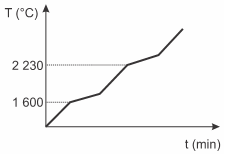
\includegraphics[width=.8\linewidth]{provas/2ano3bim2021/ImagemQ41.png}\\
			\choice .\\ 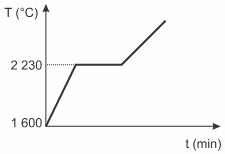
\includegraphics[width=.8\linewidth]{provas/2ano3bim2021/ImagemQ42}\\
			\choice .\\ 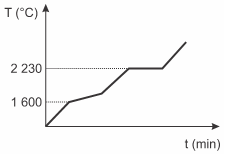
\includegraphics[width=.8\linewidth]{provas/2ano3bim2021/ImagemQ43}\\
			\choice .\\ 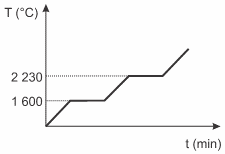
\includegraphics[width=.8\linewidth]{provas/2ano3bim2021/ImagemQ44}\\
			\choice .\\ 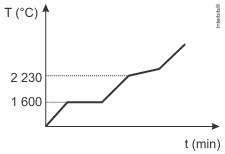
\includegraphics[width=.8\linewidth]{provas/2ano3bim2021/ImagemQ45}\\
			\end{choices}
		\end{multicols}
	\end{EnvUplevel}







